\section{Logarithmusfunktionen – Die Welt des 'Zurückrechnens'}
\label{sec:logarithmusfunktionen_intro}

Nachdem wir die Exponentialfunktionen, insbesondere die natürliche Exponentialfunktion $f(x)=e^x$, kennengelernt haben, die uns exponentielles Wachstum und Zerfall beschreiben, wenden wir uns nun ihrer direkten 'Partnerin' zu: der \textbf{Logarithmusfunktion}.

\begin{tcolorbox}[colback=blue!5!white, colframe=blue!75!black, title=Was du in diesem Kapitel lernen wirst:]
Nachdem du dieses Kapitel durchgearbeitet hast, wirst du in der Lage sein:
\begin{itemize}[noitemsep, topsep=0pt, leftmargin=*, itemsep=2pt]
    \item den \textbf{Logarithmus} allgemein als Antwort auf die Frage nach dem Exponenten zu verstehen und den \textbf{natürlichen Logarithmus ($\ln x$)} als Umkehrfunktion der natürlichen Exponentialfunktion $e^x$ zu definieren und seine grundlegenden Eigenschaften (Graph, Definitions-/Wertebereich, Nullstelle, senkrechte Asymptote, Monotonie, Krümmung) zu beschreiben.
    \item die wichtigen \textbf{Logarithmengesetze} (für Produkte, Quotienten und Potenzen) sicher anzuwenden, um logarithmische Terme zu vereinfachen und Exponentialgleichungen nach der gesuchten Variablen aufzulösen.
    \item die \textbf{Ableitung} des natürlichen Logarithmus ($(\ln x)' = 1/x$) zu kennen und die Kettenregel zur Ableitung verketteter Logarithmusfunktionen ($(\ln(h(x)))' = \frac{h'(x)}{h(x)}$) sowie Produkt- und Quotientenregel auf Funktionen mit $\ln(x)$ anzuwenden.
    \item die \textbf{Stammfunktionen} $\int \frac{1}{x} \,dx = \ln|x|+C$ und $\int \ln(x) \,dx = x\ln(x) - x + C$ (letztere mithilfe partieller Integration) zu kennen und für Berechnungen zu nutzen.
    \item Integrale der wichtigen Form $\int \frac{g'(x)}{g(x)} \,dx = \ln|g(x)|+C$ zu erkennen und zu lösen (Integration durch Substitution).
    \item eine vollständige \textbf{Kurvendiskussion} für Funktionen durchzuführen, die den natürlichen Logarithmus enthalten (oft in Produkt- oder Quotientenform mit Polynomen), unter besonderer Berücksichtigung des Definitionsbereichs und relevanter Grenzwerte (z.B. $\lim_{x \to 0^+} x^n \ln x$).
    \item die Bedeutung und Anwendung des Logarithmus in verschiedenen Kontexten zu verstehen, beispielsweise beim Lösen von Exponentialgleichungen, die bei Wachstums- und Zerfallsprozessen auftreten, oder beim Verständnis logarithmischer Skalen.
\end{itemize}
Du wirst damit die wichtige 'Partnerfunktion' der Exponentialfunktion meistern und dein analytisches Repertoire zur Untersuchung und Beschreibung von Funktionen und realen Phänomenen entscheidend erweitern!
\end{tcolorbox}
\bigskip

Stell dir vor, du hast eine Exponentialgleichung wie $e^x = 10$. Wie findest du heraus, welchen Wert $x$ haben muss, damit diese Gleichung stimmt? Du suchst also den Exponenten, mit dem die Basis $e$ potenziert werden muss, um 10 zu erhalten. Genau diese Frage beantwortet uns der Logarithmus.

\begin{infoboxumgebung}{Was ist ein Logarithmus? Die Frage nach dem Exponenten!}
Der Logarithmus einer Zahl $y$ zu einer bestimmten Basis $b$ ist derjenige Exponent $x$, mit dem man die Basis $b$ potenzieren muss, um $y$ zu erhalten.
Man schreibt: $\log_b (y) = x \quad \Leftrightarrow \quad b^x = y$.

\textbf{Beispiele:}
\begin{itemize}
    \item $\log_2 (8) = 3$, denn $2^3 = 8$. (Der Logarithmus von 8 zur Basis 2 ist 3).
    \item $\log_{10} (100) = 2$, denn $10^2 = 100$. (Der Logarithmus von 100 zur Basis 10 ist 2).
    \item $\log_5 (25) = 2$, denn $5^2 = 25$.
\end{itemize}
Der Logarithmus 'holt den Exponenten herunter'.
\end{infoboxumgebung}

In diesem Kapitel konzentrieren wir uns hauptsächlich auf den \textbf{natürlichen Logarithmus}, der die Basis $e$ (die Eulersche Zahl) hat. Er ist die direkte Umkehrfunktion der natürlichen Exponentialfunktion $f(x)=e^x$.

\subsection{Der natürliche Logarithmus \texorpdfstring{$\ln(x)$}{ln(x)} – Die Umkehrung von \texorpdfstring{$e^x$}{e hoch x}}
\label{subsec:natuerlicher_logarithmus}

Die natürliche Exponentialfunktion $f(x)=e^x$ ist streng monoton steigend und bildet alle reellen Zahlen $\mathbb{R}$ auf die positiven reellen Zahlen $\mathbb{R}^+$ ab. Daher besitzt sie eine eindeutige Umkehrfunktion, die wir als \textbf{natürlichen Logarithmus} bezeichnen und mit $\ln(x)$ (manchmal auch $\log_e(x)$) schreiben.

\begin{merksatzumgebung}[def_ln]{Definition des natürlichen Logarithmus (\texorpdfstring{$\ln x$}{ln(x)})}
Der \textbf{natürliche Logarithmus} $\ln(x)$ ist die Umkehrfunktion der natürlichen Exponentialfunktion $e^x$.
Für $x > 0$ ist $\ln(x)$ diejenige Zahl $y$, für die gilt: $e^y = x$.
Also:
\[ y = \ln(x) \quad \Leftrightarrow \quad e^y = x \]
Wichtige Beziehungen, die sich direkt aus der Umkehreigenschaft ergeben:
\begin{itemize}
    \item $e^{\ln(x)} = x$ für alle $x > 0$.
    \item $\ln(e^x) = x$ für alle $x \in \mathbb{R}$.
\end{itemize}
Die $e$-Funktion und die $\ln$-Funktion 'neutralisieren' sich gegenseitig.
\end{merksatzumgebung}

\begin{warumwichtigumgebung}{Der natürliche Logarithmus}
Der natürliche Logarithmus ist in vielen Bereichen der Mathematik und Naturwissenschaften von fundamentaler Bedeutung:
\begin{itemize}
    \item \textbf{Lösen von Exponentialgleichungen:} Immer wenn die Unbekannte im Exponenten steht (z.B. $e^{0.5t}=100$), brauchen wir den Logarithmus, um sie 'herunterzuholen'.
    \item \textbf{Modellierung von Prozessen:} Viele natürliche Prozesse, bei denen relative Änderungen eine Rolle spielen, werden mit Logarithmen beschrieben (z.B. pH-Wert, Lautstärkepegel in Dezibel, Richterskala für Erdbeben).
    \item \textbf{Integration:} Die Stammfunktion von $\frac{1}{x}$ ist $\ln|x|$.
    \item \textbf{Theoretische Mathematik:} Er taucht in vielen wichtigen Formeln und Grenzwerten auf.
\end{itemize}
\end{warumwichtigumgebung}

\subsubsection{Graph und Eigenschaften von \texorpdfstring{$f(x)=\ln(x)$}{f(x)=ln(x)}}
Der Graph der Logarithmusfunktion $f(x)=\ln(x)$ ergibt sich durch Spiegelung des Graphen der Exponentialfunktion $g(x)=e^x$ an der Winkelhalbierenden des 1. und 3. Quadranten (der Geraden $y=x$).

\begin{merksatzumgebung}[eigenschaften_lnx]{Eigenschaften der natürlichen Logarithmusfunktion \texorpdfstring{$f(x)=\ln(x)$}{f(x)=ln(x)}}
\begin{itemize}
    \item \textbf{Definitionsbereich:} $D_f = \mathbb{R}^+ = (0, \infty)$. Man kann nur von \textbf{positiven Zahlen} den Logarithmus bilden! $\ln(0)$ und $\ln(\text{negative Zahl})$ sind nicht definiert im Reellen.
    \item \textbf{Wertebereich:} $W_f = \mathbb{R}$ (der Logarithmus kann jeden reellen Wert annehmen).
    \item \textbf{Nullstelle:} $\ln(x) = 0 \Leftrightarrow e^0 = x \Leftrightarrow x=1$. Die Funktion $f(x)=\ln(x)$ hat eine Nullstelle bei $x=1$. Der Graph schneidet die x-Achse bei $N(1|0)$.
    \item \textbf{Schnittpunkt mit der y-Achse:} Gibt es nicht, da $x=0$ nicht im Definitionsbereich liegt.
    \item \textbf{Monotonie:} Die Funktion $f(x)=\ln(x)$ ist für alle $x > 0$ \textbf{streng monoton steigend}.
    \item \textbf{Krümmung:} Der Graph von $f(x)=\ln(x)$ ist für alle $x > 0$ \textbf{rechtsgekrümmt} (konkav). (Die zweite Ableitung wird $f''(x) = -1/x^2$ sein, was für $x>0$ immer negativ ist).
    \item \textbf{Grenzwerte (Verhalten an den Rändern des Definitionsbereichs):}
        \begin{itemize}
            \item $\lim_{x \to \infty} \ln(x) = +\infty$ (für große positive $x$ werden die Werte beliebig groß, aber sehr langsam).
            \item $\lim_{x \to 0^+} \ln(x) = -\infty$ (nähert sich $x$ von rechts der Null, gehen die Funktionswerte gegen $-\infty$). Die y-Achse (Gerade $x=0$) ist eine \textbf{senkrechte Asymptote}.
        \end{itemize}
\end{itemize}
\end{merksatzumgebung}
\begin{center}
    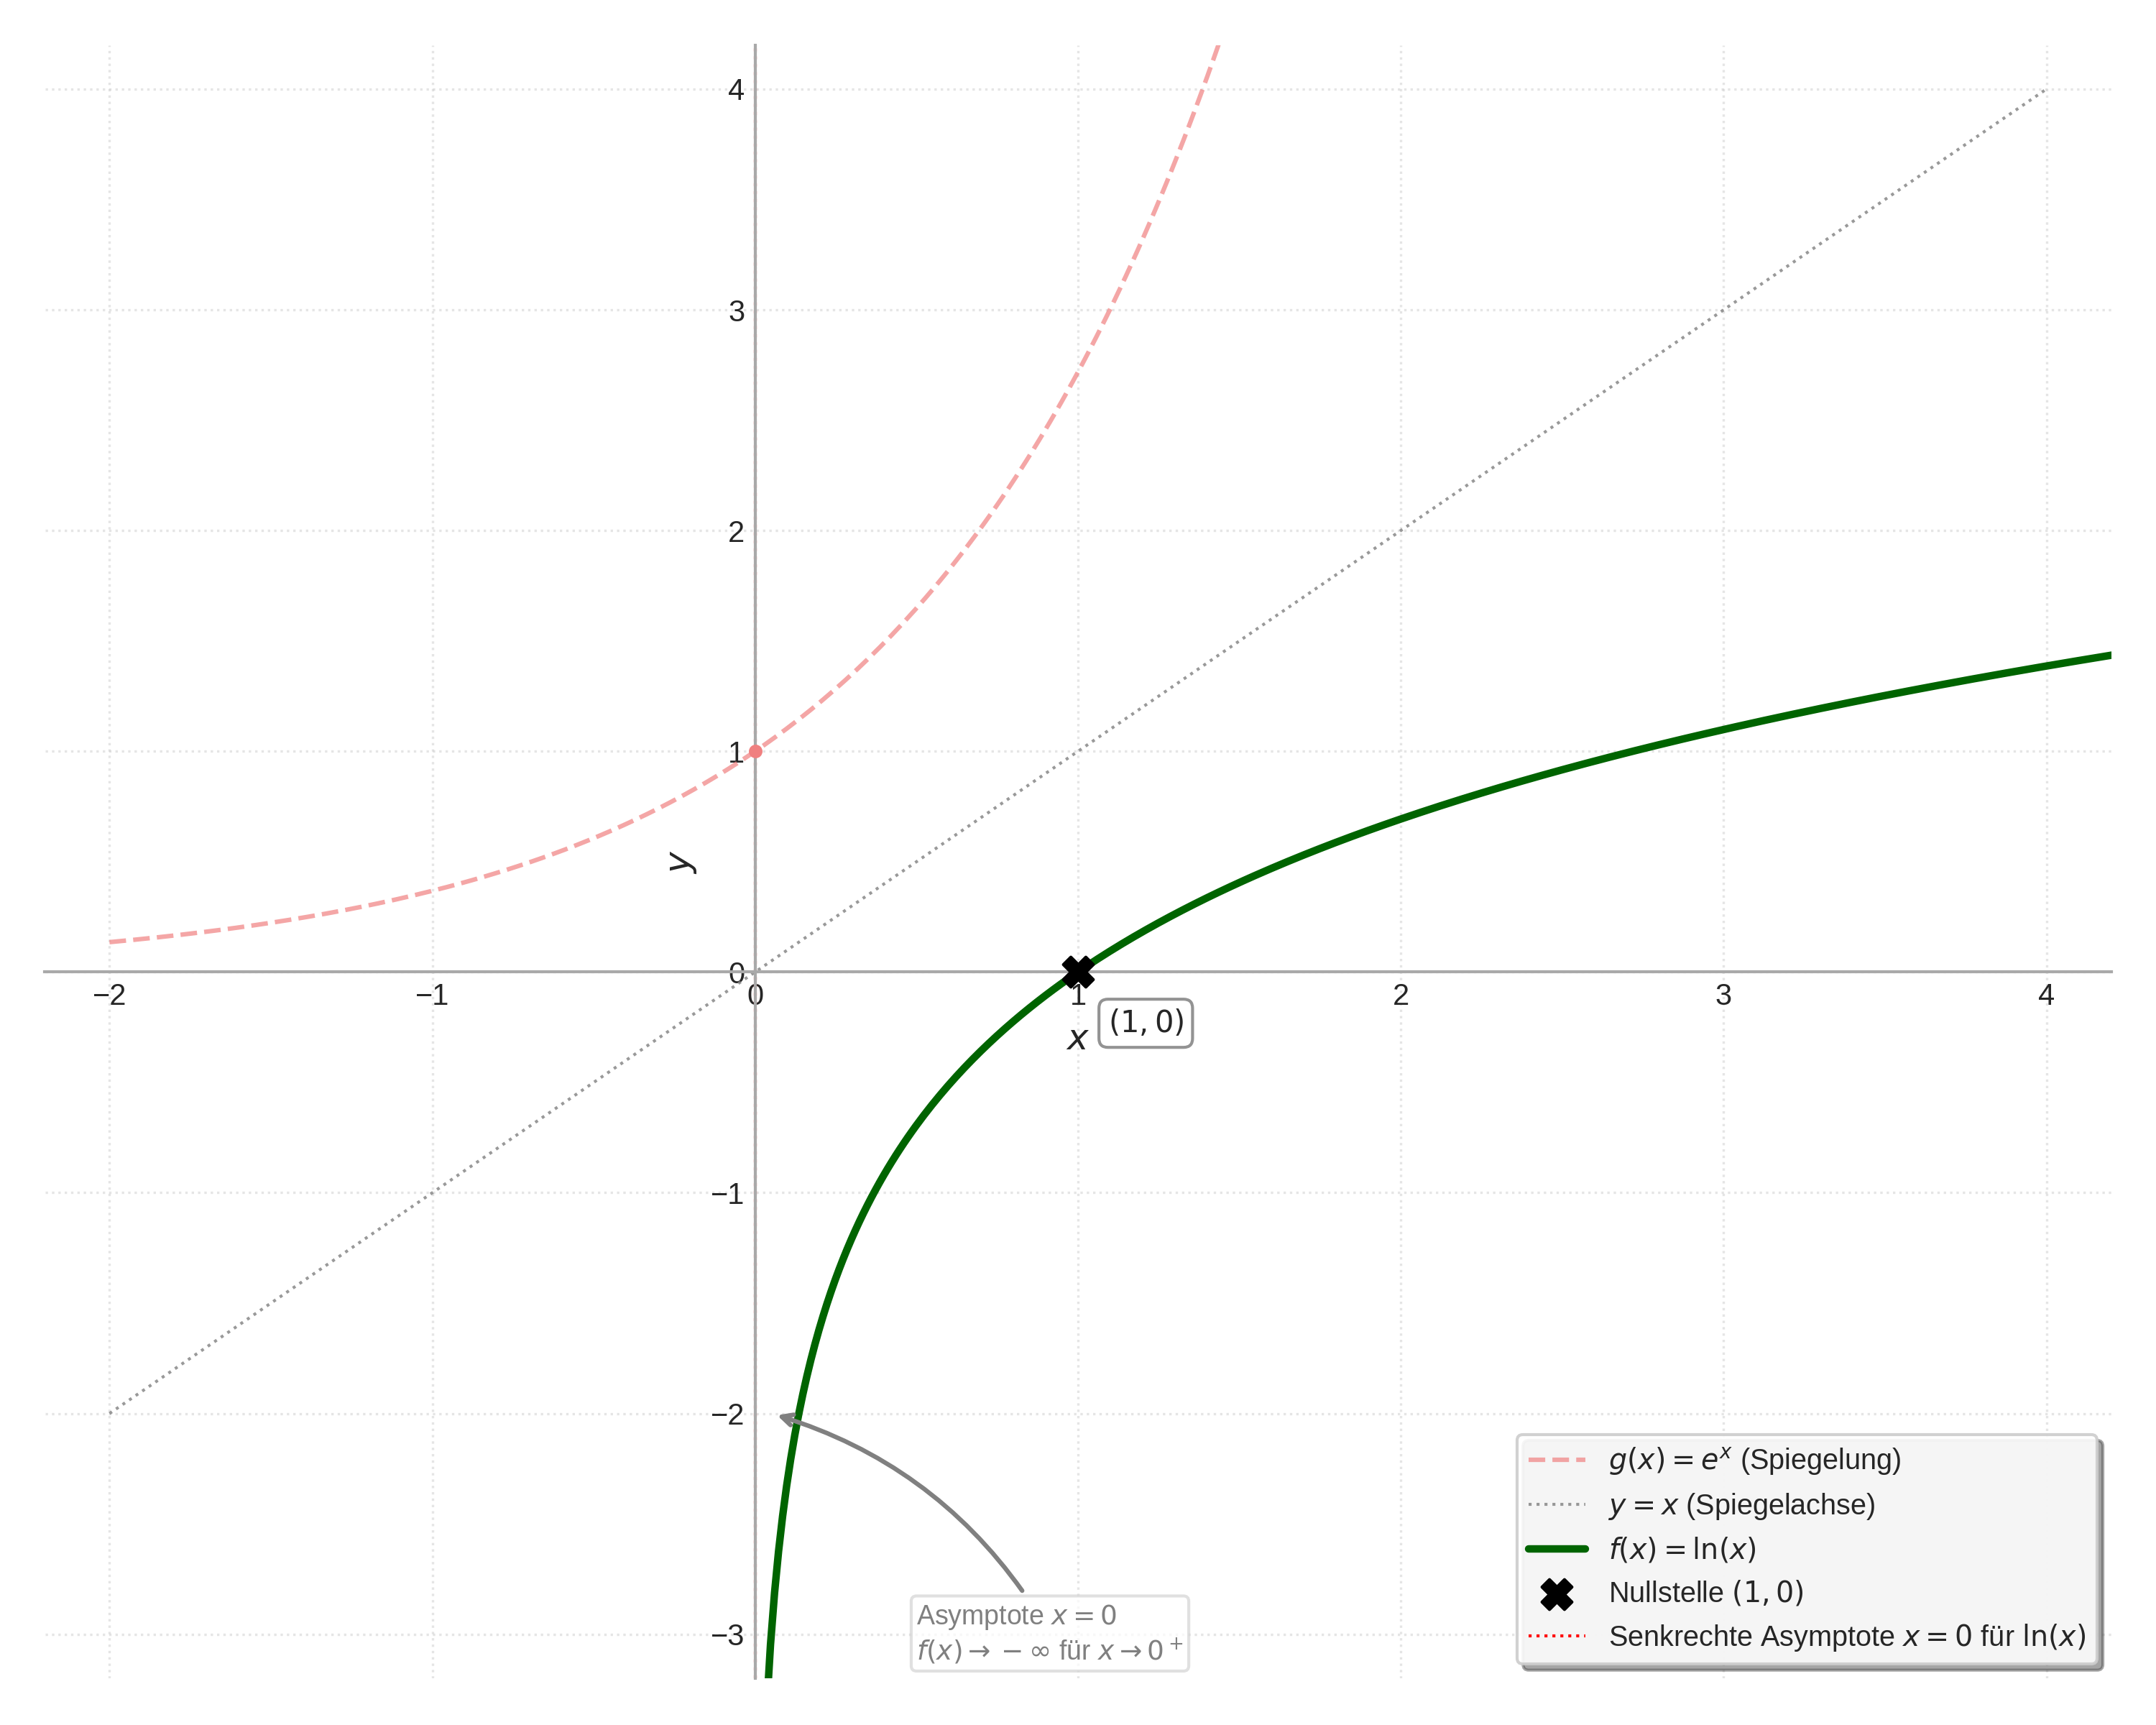
\includegraphics[width=0.8\textwidth]{grafiken/Logarithmusfunktion_lnx.png}
    \captionof{figure}{Graph der natürlichen Logarithmusfunktion \texorpdfstring{$f(x)=\ln(x)$}{f(x)=ln(x)}}
    \label{fig:log_funktion_lnx}
\end{center}
\textit{Selbst-Check:} Warum ist $\ln(1)=0$? Warum ist $\ln(e)=1$? (Antworten: Weil $e^0=1$ und $e^1=e$.)

\subsubsection{Wichtige Rechenregeln für Logarithmen (Logarithmengesetze)}
Für das Rechnen mit Logarithmen (egal zu welcher Basis) gibt es wichtige Gesetze, die sich aus den Potenzgesetzen ableiten lassen. Für den natürlichen Logarithmus lauten sie:

\begin{merksatzumgebung}[log_gesetze]{Logarithmengesetze für \texorpdfstring{$\ln(x)$}{ln(x)}}
Für $u, v > 0$ und $r \in \mathbb{R}$ gilt:
\begin{enumerate}[label=\arabic*)]
    \item \textbf{Produktregel:} $\ln(u \cdot v) = \ln(u) + \ln(v)$
    (Der Logarithmus eines Produkts ist die Summe der Logarithmen der Faktoren.)
    \item \textbf{Quotientenregel:} $\ln\left(\frac{u}{v}\right) = \ln(u) - \ln(v)$
    (Der Logarithmus eines Quotienten ist die Differenz der Logarithmen von Zähler und Nenner.)
    \item \textbf{Potenzregel:} $\ln(u^r) = r \cdot \ln(u)$
    (Der Logarithmus einer Potenz ist das Produkt aus dem Exponenten und dem Logarithmus der Basis.)
\end{enumerate}
Spezialfälle:
\begin{itemize}
    \item $\ln(e) = 1$
    \item $\ln(1) = 0$
    \item $\ln(e^x) = x$
    \item $e^{\ln(x)} = x$
\end{itemize}
\end{merksatzumgebung}

\begin{fehlerboxumgebung}{Logarithmengesetze richtig anwenden}
Die Logarithmengesetze sind mächtig, aber nur, wenn sie korrekt angewendet werden!
\begin{itemize}
    \item \textbf{Falsch:} $\ln(u+v) = \ln(u) + \ln(v)$. Der Logarithmus einer Summe ist NICHT die Summe der Logarithmen. Es gibt keine einfache Regel für $\ln(u+v)$.
    \item \textbf{Falsch:} $\ln(u-v) = \ln(u) - \ln(v)$. Analog zur Summe.
    \item \textbf{Falsch:} $\frac{\ln(u)}{\ln(v)} = \ln(u) - \ln(v)$ oder $\ln(\frac{u}{v})$. Die Division von Logarithmen ist NICHT dasselbe wie der Logarithmus eines Quotienten.
    \item \textbf{Falsch:} $(\ln(u))^r = r \ln(u)$. Die Potenzregel $\ln(u^r)=r\ln(u)$ gilt für den Logarithmus einer Potenz, nicht für eine Potenz des Logarithmus.
\end{itemize}
Überprüfe immer genau, ob du die Produkt-, Quotienten- oder Potenzregel korrekt anwendest!
\end{fehlerboxumgebung}

\begin{beispielumgebung}[anwendung_log_gesetze]{Anwendung der Logarithmengesetze}
\begin{enumerate}
    \item Vereinfache $\ln(2a) + \ln(3b) - \ln(6ab^2)$ für $a,b > 0$.
    $\ln(2a) + \ln(3b) - \ln(6ab^2) = \ln(2 \cdot a \cdot 3 \cdot b) - \ln(6ab^2)$ (Produktregel)
    $= \ln(6ab) - \ln(6ab^2)$
    $= \ln\left(\frac{6ab}{6ab^2}\right)$ (Quotientenregel)
    $= \ln\left(\frac{1}{b}\right) = \ln(b^{-1})$
    $= -1 \cdot \ln(b) = -\ln(b)$ (Potenzregel).

    \item Löse die Gleichung $e^{2x} = 5$ nach $x$.
    Wir wenden auf beiden Seiten den natürlichen Logarithmus an:
    $\ln(e^{2x}) = \ln(5)$
    Mit $\ln(e^A)=A$ folgt:
    $2x = \ln(5)$
    $x = \frac{\ln(5)}{2}$.
    Mit dem Taschenrechner: $\ln(5) \approx 1.609$, also $x \approx \frac{1.609}{2} \approx 0.8045$.
\end{enumerate}
\end{beispielumgebung}

\begin{aufgabenumgebung}{Rechnen mit Logarithmen}
\begin{enumerate}
    \item Vereinfache die folgenden Terme so weit wie möglich (alle Variablen seien positiv):
        \begin{itemize}
            \item $\ln(x^3) + \ln(x^2)$
            \item $\ln(a^5) - \ln(a^2)$
            \item $2\ln(u) - 3\ln(v)$
            \item $\frac{1}{2}\ln(16x^4)$
        \end{itemize}
    \item Löse die folgenden Exponentialgleichungen nach $x$. Gib das Ergebnis sowohl exakt als auch als Dezimalzahl (auf 3 Nachkommastellen gerundet) an.
        \begin{itemize}
            \item $e^x = 20$
            \item $2e^{3x} = 18$
            \item $e^{-0.5x+1} = 5$
            \item $100 \cdot (0.7)^x = 10$ (Tipp: Erst isolieren, dann logarithmieren. Du kannst hier $\ln$ verwenden, obwohl die Basis $0.7$ ist.)
        \end{itemize}
\end{enumerate}
\end{aufgabenumgebung}

\subsubsection{Ableitung und Stammfunktion des natürlichen Logarithmus}
\label{subsubsec:ableitung_stammfunktion_lnx}

Nachdem wir die grundlegenden Eigenschaften und Rechenregeln des natürlichen Logarithmus kennengelernt haben, wollen wir uns nun seiner Ableitung und seiner Rolle als Stammfunktion widmen.

\begin{merksatzumgebung}[ableitung_lnx]{Ableitung von \texorpdfstring{$f(x) = \ln(x)$}{f(x) = ln(x)}}
Die Ableitung der natürlichen Logarithmusfunktion $f(x) = \ln(x)$ für $x > 0$ ist:
\[ (\ln(x))' = \frac{1}{x} \]
\textit{Bemerkung:} Diese einfache und elegante Ableitung ist ein weiterer Grund, warum der natürliche Logarithmus in der Analysis so wichtig ist. Die Herleitung dieser Regel erfordert fortgeschrittenere Methoden (z.B. die Ableitung der Umkehrfunktion oder die Definition des Logarithmus über ein Integral), daher nehmen wir sie hier als gegeben hin.
\end{merksatzumgebung}

\begin{beispielumgebung}[anwendung_ableitung_lnx]{Ableitung von \texorpdfstring{$\ln(x)$}{ln(x)} anwenden}
\begin{enumerate}
    \item $f(x) = 5\ln(x) \implies f'(x) = 5 \cdot (\ln(x))' = 5 \cdot \frac{1}{x} = \frac{5}{x}$ (Faktorregel)
    \item $g(x) = x^2 + \ln(x) \implies g'(x) = (x^2)' + (\ln(x))' = 2x + \frac{1}{x}$ (Summenregel)
\end{enumerate}
\end{beispielumgebung}

Da die Ableitung von $\ln(x)$ gleich $\frac{1}{x}$ ist, ergibt sich direkt die Stammfunktion für $\frac{1}{x}$.

\begin{merksatzumgebung}[stammfunktion_1durchx]{Stammfunktion von \texorpdfstring{$f(x) = \frac{1}{x}$}{f(x) = 1/x}}
Die Menge aller Stammfunktionen (das unbestimmte Integral) von $f(x) = \frac{1}{x}$ ist:
\[ \int \frac{1}{x} \,dx = \ln|x| + C \]
\textbf{Wichtig:} Da der Logarithmus nur für positive Zahlen definiert ist, der Term $\frac{1}{x}$ aber auch für negative $x$ existiert, schreiben wir $\ln|x|$ (Logarithmus des Betrags von $x$), um den Definitionsbereich der Stammfunktion ($x \neq 0$) abzudecken.
\begin{itemize}
    \item Für $x > 0$ ist $|x|=x$, also $\int \frac{1}{x} \,dx = \ln(x) + C$.
    \item Für $x < 0$ ist $|x|=-x$. Die Ableitung von $\ln(-x)$ ist nach der Kettenregel $\frac{1}{-x} \cdot (-1) = \frac{1}{x}$. Also ist auch hier $\ln(-x)+C$ eine Stammfunktion.
\end{itemize}
Die Schreibweise $\ln|x|+C$ fasst beide Fälle zusammen.
\end{merksatzumgebung}

\begin{beispielumgebung}[integration_kdurchx]{Integrieren von \texorpdfstring{$\frac{k}{x}$}{k/x}}
Bestimme $\int \frac{7}{x} \,dx$.
\[ \int \frac{7}{x} \,dx = 7 \int \frac{1}{x} \,dx = 7 \ln|x| + C \]
\end{beispielumgebung}

\begin{fehlerboxumgebung}{Stammfunktion von $1/x$ – Den Betrag nicht vergessen!}
Die Stammfunktion von $f(x)=\frac{1}{x}$ ist $F(x)=\ln|x|+C$. Warum der Betrag?
\begin{itemize}
    \item Die Funktion $f(x)=\frac{1}{x}$ ist für alle $x \neq 0$ definiert (also für positive und negative $x$).
    \item Die Funktion $\ln(x)$ ist aber nur für $x>0$ definiert.
    \item Für $x<0$ ist die Funktion $\ln(-x)$ definiert, und ihre Ableitung ist $\frac{1}{-x} \cdot (-1) = \frac{1}{x}$.
    \item $\ln|x|$ fasst beide Fälle ($\ln(x)$ für $x>0$ und $\ln(-x)$ für $x<0$) korrekt zusammen.
\end{itemize}
Bei bestimmten Integralen über Intervalle, die nur positive oder nur negative $x$-Werte enthalten, kannst du den Betrag entsprechend auflösen. Bei unbestimmten Integralen ist $\ln|x|+C$ die präziseste Angabe.
\end{fehlerboxumgebung}

\begin{aufgabenumgebung}{Ableiten und Integrieren mit \texorpdfstring{$\ln(x)$}{ln(x)}}
\begin{enumerate}
    \item Bilde die erste Ableitung der folgenden Funktionen:
        \begin{itemize}
            \item $f_1(x) = -2\ln(x) + e^x$
            \item $f_2(x) = x^3 \ln(x)$ (Produktregel!)
            \item $f_3(x) = \frac{\ln(x)}{x}$ (Quotientenregel!)
        \end{itemize}
    \item Bestimme die Menge aller Stammfunktionen:
        \begin{itemize}
            \item $g_1(x) = \frac{3}{x} - 2x + 1$
            \item $g_2(x) = \frac{x^2+x-1}{x}$ (Tipp: Den Bruch zuerst aufteilen!)
        \end{itemize}
\end{enumerate}
\end{aufgabenumgebung}

\subsubsection{Ableitung von verketteten Logarithmusfunktionen: \texorpdfstring{$f(x) = \ln(h(x))$}{f(x) = ln(h(x))}}
Sehr oft tritt der Logarithmus als äußere Funktion einer Verkettung auf. Hier benötigen wir die Kettenregel: $(g(h(x)))' = g'(h(x)) \cdot h'(x)$.

Wenn $f(x) = \ln(h(x))$, dann ist:
\begin{itemize}
    \item Äußere Funktion: $g(u) = \ln(u) \implies g'(u) = \frac{1}{u}$.
    \item Innere Funktion: $h(x)$. Ihre Ableitung ist $h'(x)$.
\end{itemize}
Somit ist die Ableitung von $f(x) = \ln(h(x))$:
\[ (\ln(h(x)))' = \frac{1}{h(x)} \cdot h'(x) = \frac{h'(x)}{h(x)} \]

\begin{merksatzumgebung}[ableitung_lnhx]{Ableitung von \texorpdfstring{$\ln(h(x))$}{ln(h(x))} (Spezialfall der Kettenregel)}
Für eine differenzierbare Funktion $h(x)$ mit $h(x)>0$ gilt:
\[ (\ln(h(x)))' = \frac{h'(x)}{h(x)} \]
'Ableitung der inneren Funktion geteilt durch die innere Funktion.'
\end{merksatzumgebung}

\begin{fehlerboxumgebung}{Ableitung von $\ln(h(x))$ – Die Kettenregel beachten!}
Die Formel $(\ln(h(x)))' = \frac{h'(x)}{h(x)}$ ist eine direkte Anwendung der Kettenregel. Häufige Fehler sind:
\begin{itemize}
    \item \textbf{Innere Ableitung $h'(x)$ im Zähler vergessen:} Man schreibt nur $\frac{1}{h(x)}$.
    \item \textbf{Kehrwert falsch gebildet:} Man schreibt $h(x) \cdot h'(x)$ oder Ähnliches.
    \item \textbf{Definitionsbereich von $\ln(h(x))$ nicht beachtet:} Die Ableitung existiert nur dort, wo $h(x)>0$ ist und $h(x)$ differenzierbar ist.
\end{itemize}
Identifiziere immer klar die innere Funktion $h(x)$ und bilde ihre Ableitung $h'(x)$ korrekt.
\end{fehlerboxumgebung}

\begin{beispielumgebung}[kettenregel_lnhx]{Kettenregel mit \texorpdfstring{$\ln(h(x))$}{ln(h(x))}}
\begin{enumerate}
    \item $f(x) = \ln(x^2+1)$. (Hier ist $x^2+1$ immer positiv, also $D_f=\mathbb{R}$)
        Innere Funktion: $h(x) = x^2+1 \implies h'(x) = 2x$.
        $f'(x) = \frac{2x}{x^2+1}$.

    \item $g(x) = \ln(3x-5)$. (Definiert für $3x-5 > 0 \implies 3x > 5 \implies x > 5/3$)
        Innere Funktion: $h(x) = 3x-5 \implies h'(x) = 3$.
        $g'(x) = \frac{3}{3x-5}$.

    \item $k(x) = ( \ln(x) )^3$. (Definiert für $x>0$)
        Hier ist die \textbf{äußere Funktion} $g(u)=u^3$ und die \textbf{innere Funktion} $h(x)=\ln(x)$.
        $g'(u) = 3u^2$.
        $h'(x) = \frac{1}{x}$.
        $k'(x) = g'(h(x)) \cdot h'(x) = 3(\ln(x))^2 \cdot \frac{1}{x} = \frac{3(\ln x)^2}{x}$.
\end{enumerate}
\end{beispielumgebung}

\begin{aufgabenumgebung}{Kettenregel mit \texorpdfstring{$\ln(h(x))$}{ln(h(x))} üben}
Bilde die erste Ableitung der folgenden Funktionen. Gib auch den maximalen Definitionsbereich an.
\begin{enumerate}
    \item $f_1(x) = \ln(5x)$
    \item $f_2(x) = \ln(x^3+x)$ (für $x>0$)
    \item $f_3(x) = x \cdot \ln(2x+1)$ (Produkt- und Kettenregel!)
    \item $f_4(x) = e^{\ln(x^2)}$ (Tipp: Vereinfache zuerst mit den Logarithmus-/Exponentialgesetzen! Was ist $e^{\ln A}$?)
\end{enumerate}
\end{aufgabenumgebung}

\subsection{Kurvendiskussion von Funktionen mit \texorpdfstring{$\ln(x)$}{ln(x)}}
\label{subsec:kurvendiskussion_lnx}

Funktionen, die den natürlichen Logarithmus enthalten (oft in Kombination mit Polynomen), können interessante Verläufe aufweisen. Die Schritte der Kurvendiskussion bleiben dieselben, aber wir müssen die speziellen Eigenschaften des Logarithmus (Definitionsbereich, Grenzwerte) beachten.

\begin{infoboxumgebung}{Wichtige Grenzwerte mit \texorpdfstring{$\ln(x)$}{ln(x)}}
Für das Verhalten von Funktionen mit $\ln(x)$ im Unendlichen sind folgende Grenzwerte oft nützlich:
\begin{itemize}
    \item $\lim_{x \to \infty} \frac{\ln(x)}{x^n} = 0$ für jedes $n > 0$. (Jede noch so kleine positive Potenz von $x$ wächst schneller als $\ln(x)$.)
    \item $\lim_{x \to 0^+} x^n \ln(x) = 0$ für jedes $n > 0$. (Für $x \to 0^+$ geht $\ln(x) \to -\infty$, aber $x^n$ geht 'schneller' gegen $0$.)
\end{itemize}
Diese Regeln helfen zu verstehen, welcher Teil einer Funktion (z.B. in einem Produkt $x \cdot \ln x$) das Verhalten für $x \to \infty$ oder $x \to 0^+$ dominiert.
\end{infoboxumgebung}

\begin{beispielumgebung}[beispiel_kurvendisk_xlnx]{Kurvendiskussion mit \texorpdfstring{$\ln x$}{ln(x)} – Untersuchung von \texorpdfstring{$f(x) = x \ln(x)$}{f(x) = x ln(x)}}
\begin{enumerate}
    \item \textbf{Definitionsbereich:} Wegen $\ln(x)$ muss $x>0$ sein. Also $D_f = (0, \infty) = \mathbb{R}^+$.
    \item \textbf{Symmetrie:} Da $D_f$ nicht symmetrisch zum Ursprung ist, kann keine einfache Symmetrie vorliegen.
    \item \textbf{Verhalten an den Rändern des Definitionsbereichs:}
        \begin{itemize}
            \item Für $x \to \infty$: $x \to \infty$ und $\ln(x) \to \infty$. Also $\lim_{x \to \infty} x \ln(x) = +\infty$.
            \item Für $x \to 0^+$: $x \to 0$ und $\ln(x) \to -\infty$. Wir haben einen Typ '$0 \cdot (-\infty)$'.
            Mit dem oben genannten Grenzwert $\lim_{x \to 0^+} x^n \ln(x) = 0$ (hier für $n=1$) gilt:
            $\lim_{x \to 0^+} x \ln(x) = 0$.
            Der Graph nähert sich also dem Ursprung $(0|0)$ für $x \to 0^+$.
        \end{itemize}
    \item \textbf{y-Achsenabschnitt:} Gibt es nicht, da $x=0$ nicht im Definitionsbereich ist.
    \item \textbf{Nullstellen:} $f(x)=0 \implies x \ln(x) = 0$.
        Da $x>0$ im Definitionsbereich, kann $x$ nicht Null sein. Also muss $\ln(x)=0$ sein.
        $\ln(x)=0 \implies x = e^0 = 1$.
        Einzige Nullstelle bei $N(1|0)$.
    \item \textbf{Erste Ableitung $f'(x)$:} Mit Produktregel $u(x)=x, u'(x)=1, v(x)=\ln(x), v'(x)=1/x$.
        $f'(x) = 1 \cdot \ln(x) + x \cdot \frac{1}{x} = \ln(x) + 1$.
    \item \textbf{Extremstellen:} $f'(x)=0 \implies \ln(x) + 1 = 0 \implies \ln(x) = -1$.
        $x_E = e^{-1} = \frac{1}{e} \approx 0.368$.
    \item \textbf{Zweite Ableitung $f''(x)$:} $f''(x) = (\ln(x)+1)' = \frac{1}{x} + 0 = \frac{1}{x}$.
    \item \textbf{Art der Extremstelle bei $x_E=1/e$ mit $f''$ prüfen:}
        $f''(1/e) = \frac{1}{1/e} = e$.
        Da $f'(1/e)=0$ und $f''(1/e)=e > 0 \implies$ Lokaler Tiefpunkt bei $x_E=1/e$.
        $y_T = f(1/e) = \frac{1}{e} \ln(\frac{1}{e}) = \frac{1}{e} \ln(e^{-1}) = \frac{1}{e} \cdot (-1) = -\frac{1}{e} \approx -0.368$.
        Tiefpunkt $T(1/e | -1/e)$.
    \item \textbf{Monotonie:} Nullstelle von $f'(x)=\ln(x)+1$ ist $x=1/e$.
        \begin{itemize}
            \item $0 < x < 1/e$ (z.B. $x=0.1 \approx 1/(2e)$): $\ln(0.1) \approx -2.3$. $f'(0.1) = -2.3+1 = -1.3 < 0 \implies$ fallend.
            \item $x > 1/e$ (z.B. $x=1$): $f'(1) = \ln(1)+1 = 0+1 = 1 > 0 \implies$ steigend.
        \end{itemize}
        Fallend für $x \in (0, 1/e]$, steigend für $x \in [1/e, \infty)$.
    \item \textbf{Wendepunkte:} $f''(x_W)=0 \implies \frac{1}{x_W}=0$. Diese Gleichung hat keine Lösung, da ein Bruch nur Null ist, wenn der Zähler Null ist (hier ist der Zähler 1). Also keine Nullstellen von $f''(x)$.
    \item \textbf{Krümmungsverhalten:} Da $D_f=(0,\infty)$, ist $x$ immer positiv. Somit ist $f''(x)=\frac{1}{x}$ immer positiv für alle $x \in D_f$.
        Der Graph ist also im gesamten Definitionsbereich linksgekrümmt (konvex). Es gibt keine Wendepunkte.
    \item \textbf{Skizze:}
        \begin{center}
            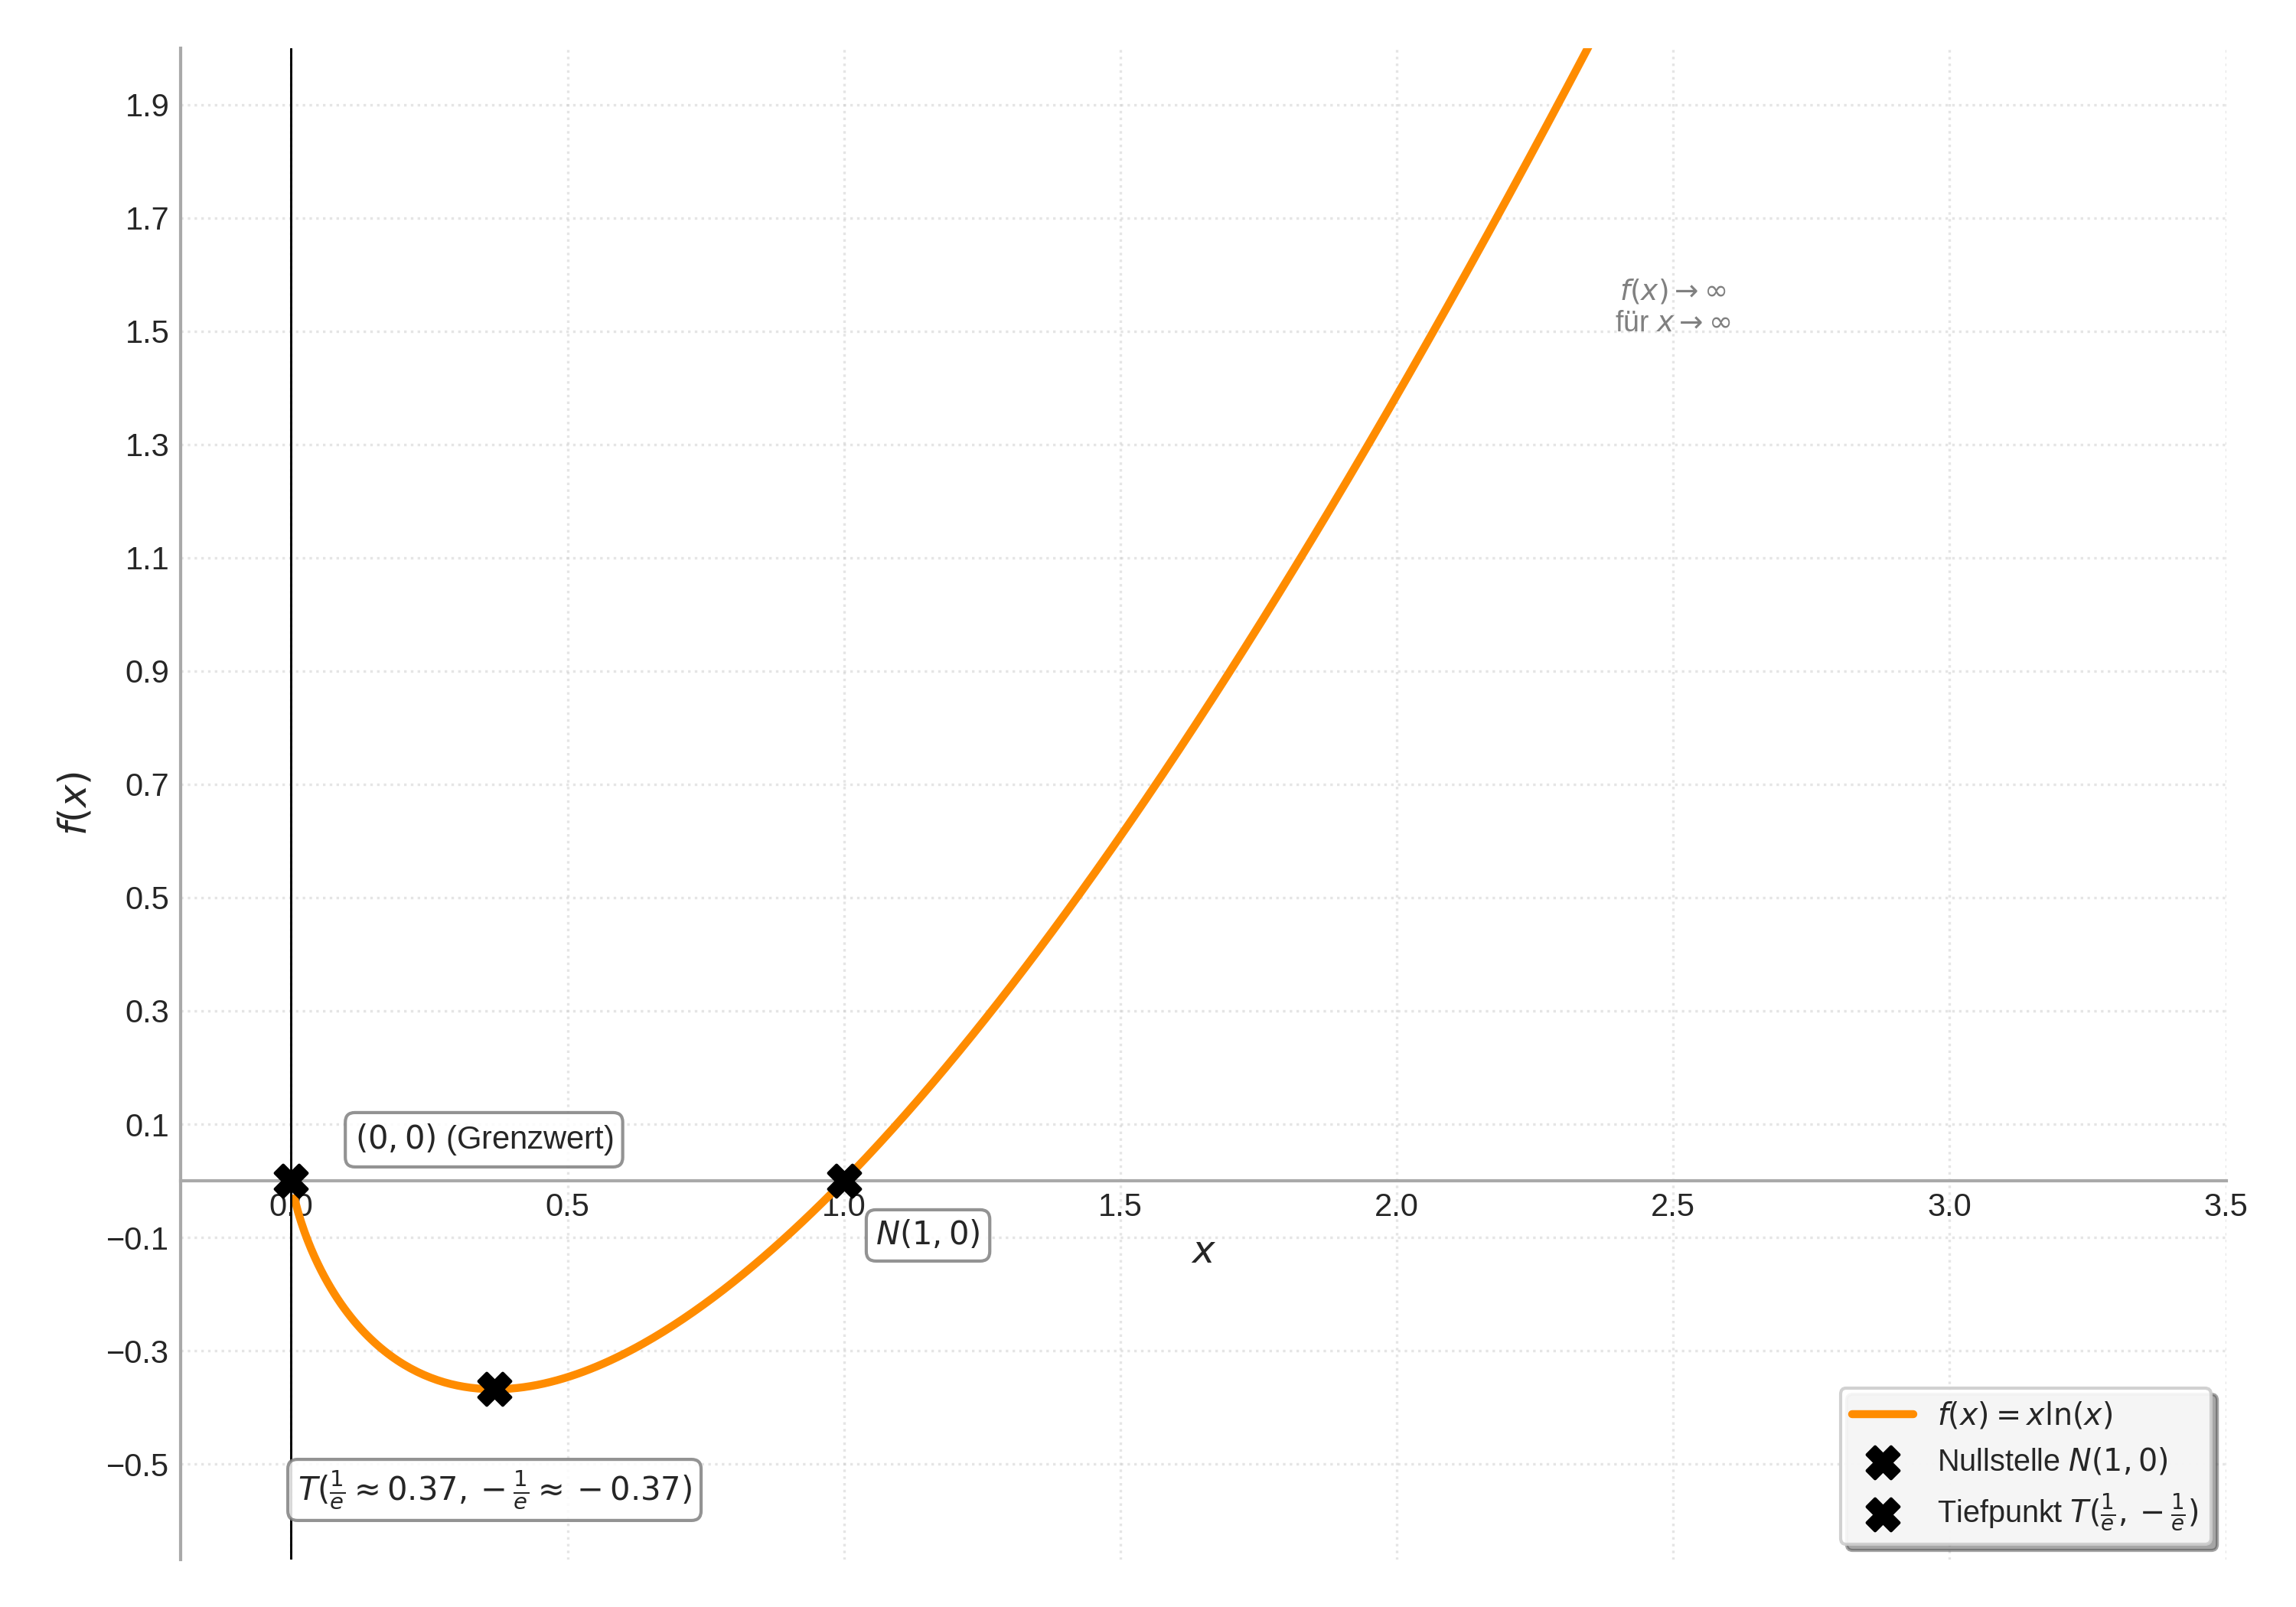
\includegraphics[width=0.9\textwidth]{grafiken/Kurvendiskussion_xlnx.png}
            \captionof{figure}{Graph von \texorpdfstring{$f(x)=x\ln(x)$}{f(x)=xln(x)}}
            \label{fig:kurvendisk_xlnx}
        \end{center}
\end{enumerate}
\end{beispielumgebung}

\begin{aufgabenumgebung}{Kurvendiskussionen mit Logarithmusfunktionen}
Führe eine vollständige Kurvendiskussion für die folgenden Funktionen durch.
\begin{enumerate}
    \item $f(x) = \ln(x^2+2)$ (Beachte den Definitionsbereich!)
    \item $g(x) = \frac{\ln x}{x}$ (für $x>0$)
    \item \textbf{Für Experten:} $h(x) = x^2 \ln(x)$ (für $x>0$)
\end{enumerate}
\end{aufgabenumgebung}

\begin{tippumgebung}{Anwendungen von Logarithmusfunktionen}
Logarithmusfunktionen sind oft die 'Antwort', wenn es um die Umkehrung exponentieller Prozesse geht oder wenn Größen über viele Zehnerpotenzen variieren.
\begin{itemize}
    \item \textbf{Halbwertszeiten/Verdopplungszeiten:} Berechnung der Zeit, bis sich eine Menge halbiert oder verdoppelt (siehe Aufgabe zum radioaktiven Zerfall im Exponentialfunktionskapitel).
    \item \textbf{Skalen:} pH-Wert (misst Säuregrad), Dezibel (Lautstärke), Richterskala (Erdbebenstärke) sind logarithmische Skalen. Eine Erhöhung um 1 auf der Skala bedeutet oft eine Verzehnfachung der eigentlichen physikalischen Größe.
    \item \textbf{Wachstumsmodelle:} Manchmal ist es einfacher, das logarithmierte Wachstum zu analysieren.
\end{itemize}
\end{tippumgebung}

\subsubsection{Integration mit Logarithmusfunktionen – Partielle Integration und ein wichtiger Spezialfall der Substitution}
\label{subsubsec:integration_lnx_neu}

Wir wissen bereits, dass die Stammfunktion von $f(x)=\frac{1}{x}$ die Funktion $F(x)=\ln|x|+C$ ist. Aber wie integriert man die Logarithmusfunktion $\ln(x)$ selbst? Und gibt es spezielle Strukturen bei Integralen, die auf Logarithmen führen?

\textbf{1. Die Stammfunktion von $\ln(x)$ – Ein Fall für die partielle Integration}

Um $\int \ln(x) \,dx$ zu berechnen, verwenden wir einen kleinen Trick und die partielle Integration.
Erinnerung Partielle Integration: $\int u'(x)v(x) \,dx = u(x)v(x) - \int u(x)v'(x) \,dx$.

Wir schreiben $\ln(x)$ als Produkt: $\ln(x) = 1 \cdot \ln(x)$.
Nun wählen wir geschickt:
\begin{itemize}
    \item $u'(x) = 1 \implies u(x) = \int 1 \,dx = x$
    \item $v(x) = \ln(x) \implies v'(x) = \frac{1}{x}$
\end{itemize}
Einsetzen in die Formel der partiellen Integration:
\begin{align*} \int \underbrace{1}_{u'(x)} \cdot \underbrace{\ln(x)}_{v(x)} \,dx &= \underbrace{x}_{u(x)} \cdot \underbrace{\ln(x)}_{v(x)} - \int \underbrace{x}_{u(x)} \cdot \underbrace{\frac{1}{x}}_{v'(x)} \,dx \\ &= x \ln(x) - \int 1 \,dx \\ &= x \ln(x) - x + C \end{align*}

\begin{merksatzumgebung}[stammfunktion_lnx]{Stammfunktion von $\ln(x)$}
Die Menge aller Stammfunktionen (das unbestimmte Integral) von $f(x) = \ln(x)$ für $x>0$ ist:
\[ \int \ln(x) \,dx = x \ln(x) - x + C \]
Oder ausgeklammert: $\int \ln(x) \,dx = x(\ln(x) - 1) + C$.
Diese wichtige Stammfunktion solltest du dir merken!
\end{merksatzumgebung}

\begin{beispielumgebung}[best_integral_lnx]{Bestimmtes Integral von \texorpdfstring{$\ln(x)$}{ln(x)}}
Berechne $\int_1^e \ln(x) \,dx$.
Wir verwenden die Stammfunktion $F(x) = x\ln(x) - x$:
\begin{align*} \int_1^e \ln(x) \,dx &= [x\ln(x) - x]_1^e \\ &= (e \cdot \ln(e) - e) - (1 \cdot \ln(1) - 1) \\ &= (e \cdot 1 - e) - (1 \cdot 0 - 1) && \text{(da } \ln(e)=1 \text{ und } \ln(1)=0) \\ &= (e - e) - (0 - 1) \\ &= 0 - (-1) = 1 \end{align*}
Der Flächeninhalt unter dem Graphen von $\ln(x)$ zwischen $x=1$ und $x=e$ beträgt also genau 1.
\begin{center}
    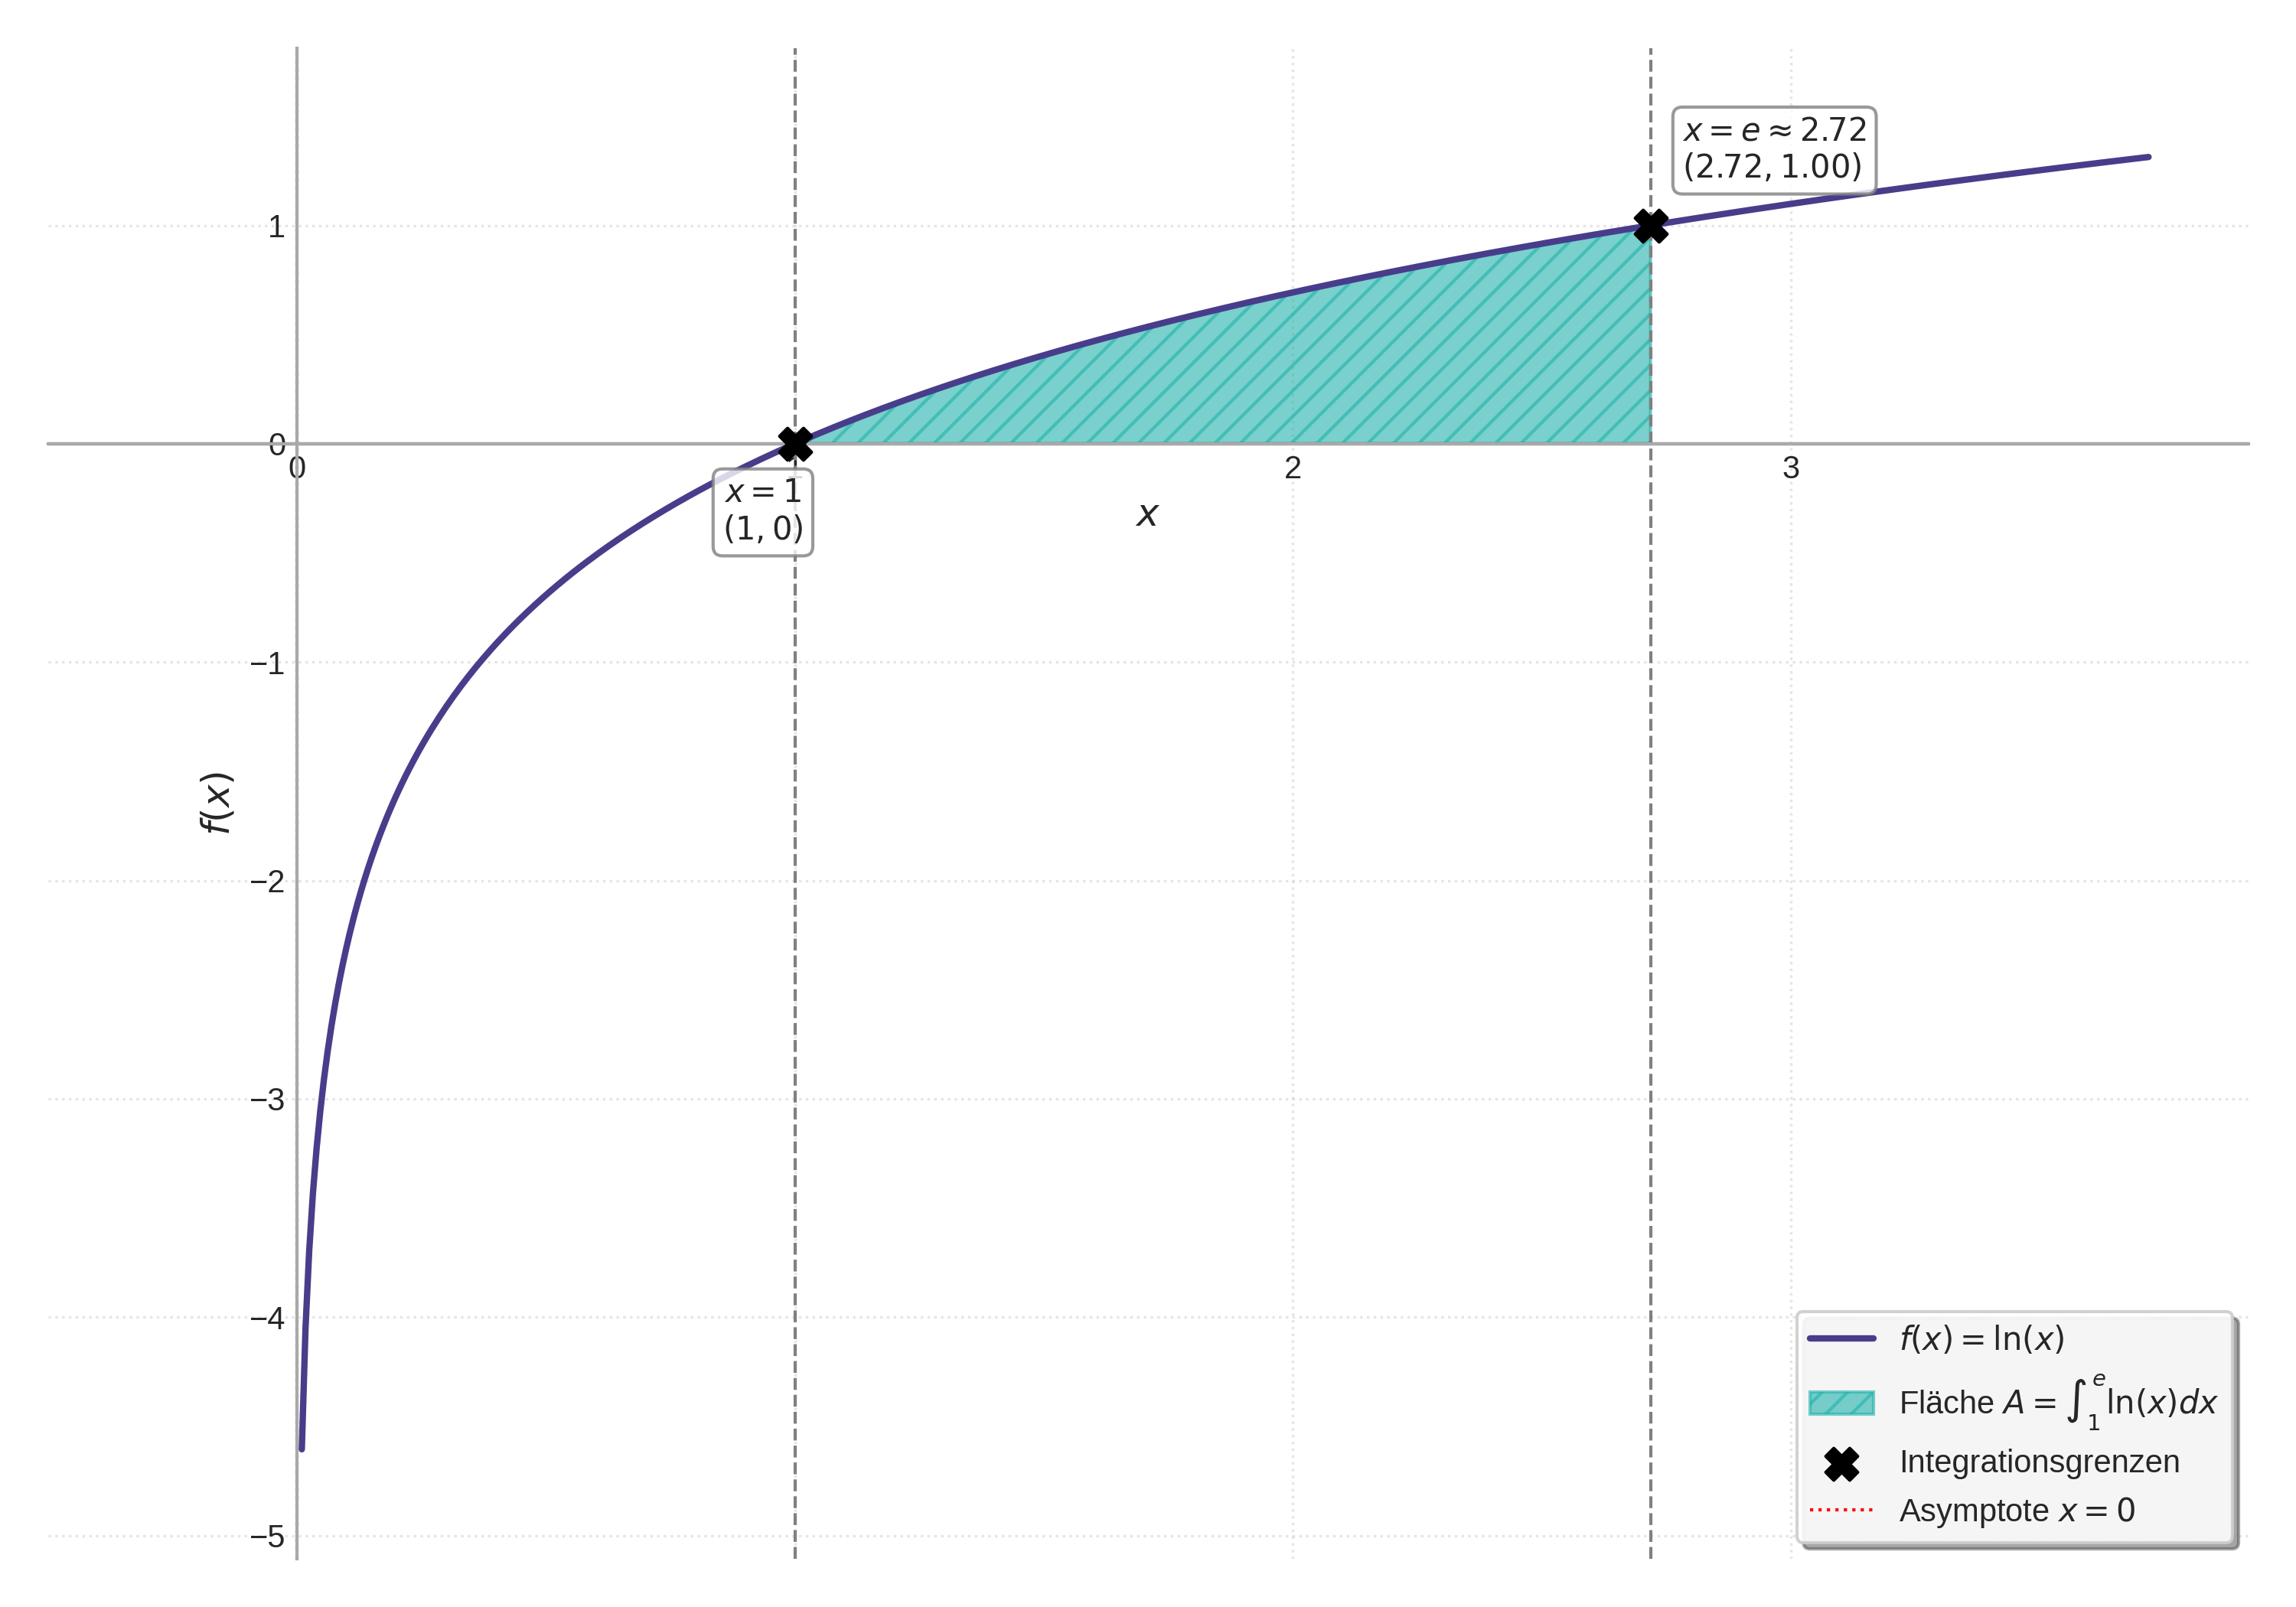
\includegraphics[width=0.8\textwidth]{grafiken/Integral_Flaeche_lnx.png}
    \captionof{figure}{Fläche unter \texorpdfstring{$f(x)=\ln(x)$}{f(x)=ln(x)} von $x=1$ bis $x=e$}
    \label{fig:flaeche_lnx}
\end{center}
\end{beispielumgebung}

\textbf{2. Ein wichtiger Spezialfall der Substitution: $\int \frac{g'(x)}{g(x)} \,dx$}

Betrachten wir Integrale, bei denen der Zähler die Ableitung des Nenners ist (oder ein Vielfaches davon).
Also Integrale der Form $\int \frac{g'(x)}{g(x)} \,dx$.

Hier hilft die Substitution $u = g(x)$.
Dann ist $\frac{du}{dx} = g'(x)$, also $du = g'(x)dx$.
Setzen wir das ins Integral ein:
\[ \int \frac{g'(x)}{g(x)} \,dx = \int \frac{1}{g(x)} \cdot g'(x)dx = \int \frac{1}{u} \,du \]
Das Integral von $\frac{1}{u}$ ist $\ln|u|+C$.
Rücksubstituieren wir $u=g(x)$, erhalten wir:

\begin{merksatzumgebung}[integration_gstrich_durch_g]{Integration von $\frac{\text{Ableitung}}{\text{Funktion}}$}
Für eine differenzierbare Funktion $g(x)$ mit $g(x) \neq 0$ gilt:
\[ \int \frac{g'(x)}{g(x)} \,dx = \ln|g(x)| + C \]
Diese Regel ist sehr nützlich und erspart oft die explizite Durchführung der Substitution.
\end{merksatzumgebung}

\begin{beispielumgebung}[anwendung_int_gstrich_g]{Anwendung der Regel \texorpdfstring{$\int \frac{g'(x)}{g(x)} \,dx$}{Integral g'(x)/g(x) dx}}
\begin{enumerate}
    \item \textbf{Integral $\int \frac{2x}{x^2+1} \,dx$}
        Sei $g(x) = x^2+1$. Dann ist $g'(x) = 2x$.
        Der Integrand hat genau die Form $\frac{g'(x)}{g(x)}$.
        Also: $\int \frac{2x}{x^2+1} \,dx = \ln|x^2+1| + C$.
        Da $x^2+1$ immer positiv ist, können wir die Betragsstriche weglassen: $\ln(x^2+1) + C$.

    \item \textbf{Integral $\int \frac{x}{x^2-4} \,dx$}
        Sei $g(x) = x^2-4$. Dann ist $g'(x) = 2x$.
        Im Zähler steht $x$, wir bräuchten aber $2x$. Wir können den Integranden mit $\frac{2}{2}$ erweitern:
        $\int \frac{x}{x^2-4} \,dx = \int \frac{1}{2} \cdot \frac{2x}{x^2-4} \,dx = \frac{1}{2} \int \frac{2x}{x^2-4} \,dx$.
        Jetzt hat der Bruch die Form $\frac{g'(x)}{g(x)}$.
        Also: $\frac{1}{2} \ln|x^2-4| + C$.
\end{enumerate}
\end{beispielumgebung}

\begin{aufgabenumgebung}{Integration mit Logarithmusfunktionen üben}
\begin{enumerate}
    \item Berechne die folgenden unbestimmten Integrale:
        \begin{itemize}
            \item $\int (3\ln(x) - 2x) \,dx$
            \item $\int \frac{5x^4}{x^5+1} \,dx$
            \item $\int \frac{e^x}{e^x+3} \,dx$
            \item $\int \frac{1}{2x+7} \,dx$ (Tipp: Erweitere so, dass der Zähler die Ableitung des Nenners ist.)
        \end{itemize}
    \item \textbf{Flächenberechnung:}
        Die Funktion $f(x) = \frac{1}{x}$ ist im ersten Quadranten gegeben.
        \begin{itemize}
            \item Berechne den Inhalt der Fläche, die der Graph von $f(x)$ mit der x-Achse im Intervall $[1, e]$ einschließt.
            \item Berechne den Inhalt der Fläche, die der Graph von $f(x)$ mit der x-Achse im Intervall $[1, b]$ für ein beliebiges $b>1$ einschließt. Was passiert mit dieser Fläche, wenn $b \to \infty$? (Uneigentliches Integral)
        \end{itemize}
    \item \textbf{Anwendung partielle Integration (anspruchsvoller):}
        Berechne $\int x^2 \ln(x) \,dx$. (Tipp: Wähle $v(x)=\ln(x)$ und $u'(x)=x^2$).
\end{enumerate}
\end{aufgabenumgebung}

\begin{kurzknappumgebung}{Logarithmusfunktionen – Analysis im Überblick}
\begin{itemize}
    \item \textbf{Natürlicher Logarithmus $\ln(x)$:} Umkehrfunktion von $e^x$. $D_f=(0,\infty)$, $W_f=\mathbb{R}$. Nullstelle bei $x=1$. Senkrechte Asymptote $x=0$.
    \item \textbf{Logarithmengesetze:} Helfen beim Umformen von Termen mit Logarithmen.
    \item \textbf{Ableitung:} $(\ln x)' = \frac{1}{x}$. Für verkettete Funktionen: $(\ln(h(x)))' = \frac{h'(x)}{h(x)}$.
    \item \textbf{Stammfunktion:} $\int \frac{1}{x} \,dx = \ln|x|+C$. $\int \ln(x) \,dx = x\ln(x) - x + C$.
    \item \textbf{Wichtiger Spezialfall der Substitution:} $\int \frac{g'(x)}{g(x)} \,dx = \ln|g(x)|+C$.
    \item \textbf{Kurvendiskussion:} Beachte Definitionsbereich und Grenzwerte an den Rändern.
\end{itemize}
\end{kurzknappumgebung}

\begin{infoboxumgebung}{Ausblick: Die Reise geht weiter – Trigonometrische Funktionen}
Mit den Exponential- und Logarithmusfunktionen hast du zwei sehr wichtige nicht-polynomielle Funktionsklassen kennengelernt, die in unzähligen Bereichen der Wissenschaft und des Alltags Anwendung finden.

Als Nächstes auf unserer mathematischen Entdeckungsreise stehen die \textbf{trigonometrischen Funktionen} ($\sin x, \cos x, \tan x$) auf dem Programm. Diese periodischen Funktionen sind unerlässlich, um Schwingungen, Wellen und zyklische Vorgänge zu beschreiben – von den Gezeiten über Schallwellen bis hin zu den Bewegungen von Planeten.

Auch für diese neuen Funktionstypen werden wir lernen, wie man sie ableitet und integriert, und wie wir sie in Kurvendiskussionen und Anwendungsaufgaben nutzen können. Die Werkzeuge der Differential- und Integralrechnung, die du bisher erworben hast, werden dabei immer wieder von zentraler Bedeutung sein. Die Mathematik baut aufeinander auf – und das ist das Schöne daran!
\end{infoboxumgebung}

\begin{aufgabenumgebung}{Checkliste: Das Wesen des Logarithmus und der $\ln$-Funktion verstehen}
Der Logarithmus, insbesondere der natürliche Logarithmus $\ln(x)$, ist ein Schlüsselkonzept mit vielen Facetten. Diese Fragen helfen dir, die Grundlagen zu festigen:

\begin{enumerate}[label=(\alph*)]
    \item \textbf{Definition und Umkehrbeziehung:}
    \begin{itemize}
        \item Erkläre mit eigenen Worten, was $\log_b(y)=x$ bedeutet. Was ist die spezielle Basis beim natürlichen Logarithmus $\ln(x)$?
        \item Warum muss gelten: $e^{\ln(x)} = x$ (für $x>0$) und $\ln(e^x) = x$ (für alle $x \in \mathbb{R}$)? Erläutere dies am Konzept der Umkehrfunktion.
        \item Begründe, warum $\ln(1)=0$ und $\ln(e)=1$ sein muss.
    \end{itemize}
    \item \textbf{Definitionsbereich und Graph:}
    \begin{itemize}
        \item Warum ist der Definitionsbereich der Funktion $f(x)=\ln(x)$ auf positive reelle Zahlen ($x>0$) beschränkt? Wie hängt das mit dem Wertebereich der $e$-Funktion zusammen?
        \item Beschreibe die wesentlichen Unterschiede im Graphenverlauf zwischen $g(x)=e^x$ und $f(x)=\ln(x)$ bezüglich Monotonie, Krümmung und Asymptoten. Wie kommt die geometrische Beziehung (Spiegelung an $y=x$) zustande?
    \end{itemize}
    \item \textbf{Logarithmengesetze anwenden und verstehen:}
    \begin{itemize}
        \item Die Regel $\ln(u^r) = r \cdot \ln(u)$ ist besonders nützlich beim Lösen von Exponentialgleichungen. Erkläre, warum diese Regel das 'Herunterholen' des Exponenten ermöglicht.
        \item Ist die Aussage $\ln(a+b) = \ln(a) + \ln(b)$ korrekt? Überprüfe mit einem Zahlenbeispiel und vergleiche mit der Produktregel $\ln(a \cdot b) = \ln(a) + \ln(b)$.
    \end{itemize}
\end{enumerate}
\end{aufgabenumgebung}

\begin{aufgabenumgebung}{Checkliste: Analysis mit der $\ln$-Funktion – Ableiten, Integrieren, Anwenden}
Die $\ln$-Funktion und ihre Ableitung $1/x$ tauchen in vielen analytischen Zusammenhängen auf.

\begin{enumerate}[label=(\alph*)]
    \item \textbf{Ableiten mit $\ln(x)$:}
    \begin{itemize}
        \item Die Ableitung von $\ln(x)$ ist $1/x$. Was sagt dir das über die Steigung des Graphen von $\ln(x)$ für $x$-Werte nahe Null (aber $x>0$) im Vergleich zu sehr großen $x$-Werten?
        \item Bei der Ableitung von $\ln(h(x))$ lautet die Regel $\frac{h'(x)}{h(x)}$. Erkläre, wie die Kettenregel hier zur Anwendung kommt ($g(u)=\ln u \implies g'(u)=1/u$).
    \end{itemize}
    \item \textbf{Integrieren mit $\ln(x)$:}
    \begin{itemize}
        \item Warum schreiben wir $\int \frac{1}{x} \,dx = \ln|x|+C$ mit Betragsstrichen, obwohl der Definitionsbereich von $\ln(x)$ selbst $x>0$ ist?
        \item Für die Berechnung von $\int \ln(x) \,dx$ wurde die partielle Integration mit $u'(x)=1$ und $v(x)=\ln(x)$ genutzt. Warum wäre die Wahl $u'(x)=\ln(x)$ und $v(x)=1$ nicht zielführend, wenn du $\int \ln(x) \,dx$ noch nicht kennst?
        \item Erkläre, warum das Integral $\int \frac{g'(x)}{g(x)} \,dx$ auf $\ln|g(x)|+C$ führt. Welche Substitution steckt dahinter?
    \end{itemize}
    \item \textbf{Kurvendiskussion und Grenzwerte:}
    \begin{itemize}
        \item Wenn du eine Funktion wie $f(x)=x^2 \ln(x)$ untersuchst: Welcher der beiden Faktoren ($x^2$ oder $\ln(x)$) 'dominiert' das Verhalten für $x \to \infty$? Und für $x \to 0^+$? (Denke an die bekannten Grenzwerte $\lim_{x \to \infty} \frac{\ln x}{x^n}=0$ und $\lim_{x \to 0^+} x^n \ln x = 0$).
        \item Welche Schritte sind bei einer Kurvendiskussion einer Funktion mit $\ln(x)$ besonders wichtig im Hinblick auf den Definitionsbereich?
    \end{itemize}
\end{enumerate}
\end{aufgabenumgebung}

